% Created 2012-04-08 Sun 09:23
\documentclass[11pt]{article}
\usepackage[utf8]{inputenc}
\usepackage[T1]{fontenc}
\usepackage{fixltx2e}
\usepackage{graphicx}
\usepackage{longtable}
\usepackage{float}
\usepackage{wrapfig}
\usepackage{soul}
\usepackage{textcomp}
\usepackage{marvosym}
\usepackage{wasysym}
\usepackage{latexsym}
\usepackage{amssymb}
\usepackage{hyperref}
\tolerance=1000
\providecommand{\alert}[1]{\textbf{#1}}

\title{Howto beamer with org-mode}
\author{Antoine R. Dumont}
\date{\today}
\hypersetup{
  pdfkeywords={},
  pdfsubject={},
  pdfcreator={Emacs Org-mode version 7.8.07}}

\begin{document}

\maketitle

\setcounter{tocdepth}{3}
\tableofcontents
\vspace*{1cm}

\section{Pre-requisites}
\label{sec-1}
\section{Install the other pre-requisites}
\label{sec-2}


\begin{verbatim}
sudo aptitude install latex latex-beamer \
  texlive-latex-extra texlive-fonts-recommended ttf-marvosym
\end{verbatim}
\section{Init a org file}
\label{sec-3}
\subsection{There is automatically a front-page}
\label{sec-3-3}

The informations comes from the previous blocks.

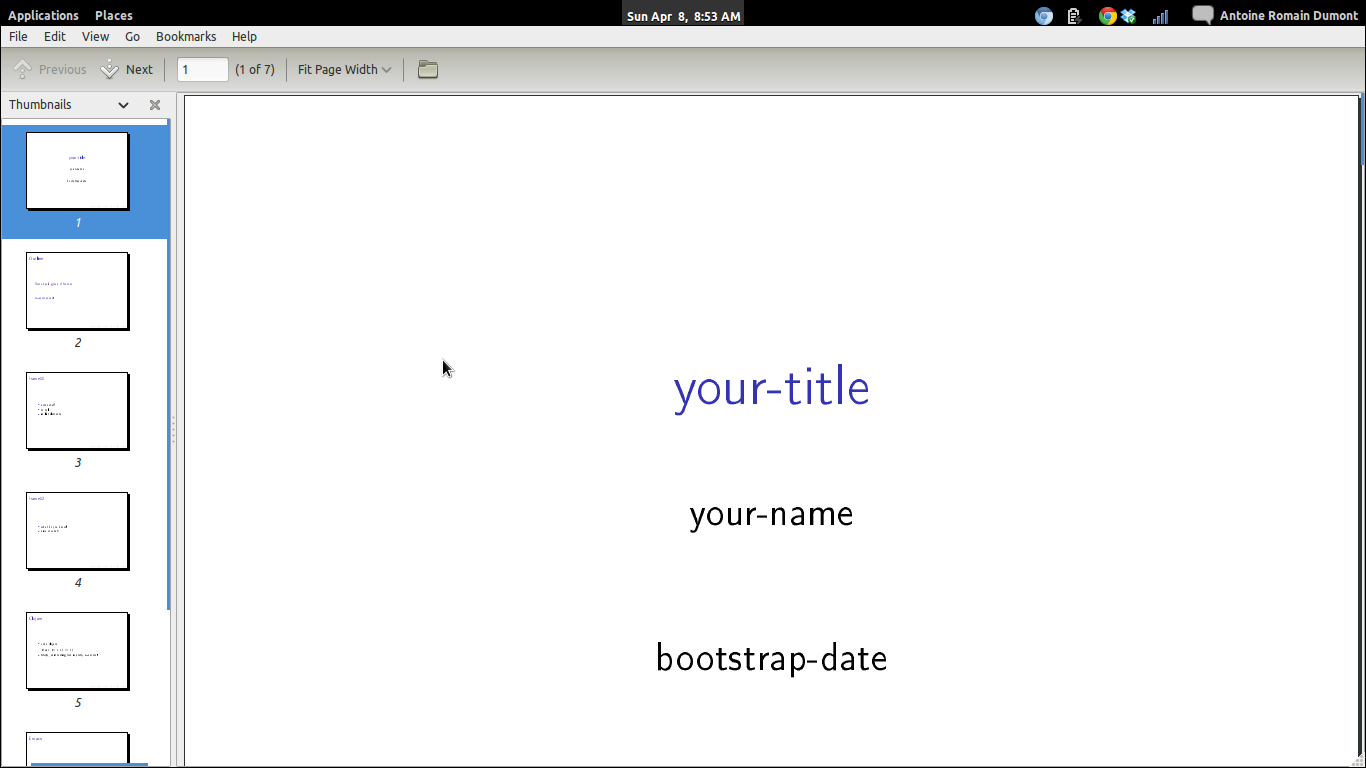
\includegraphics[width=.9\linewidth]{./org-beamer-examples/front-page.png}
\subsection{And a outline page}
\label{sec-3-4}


This will come from the content of the other frames below.

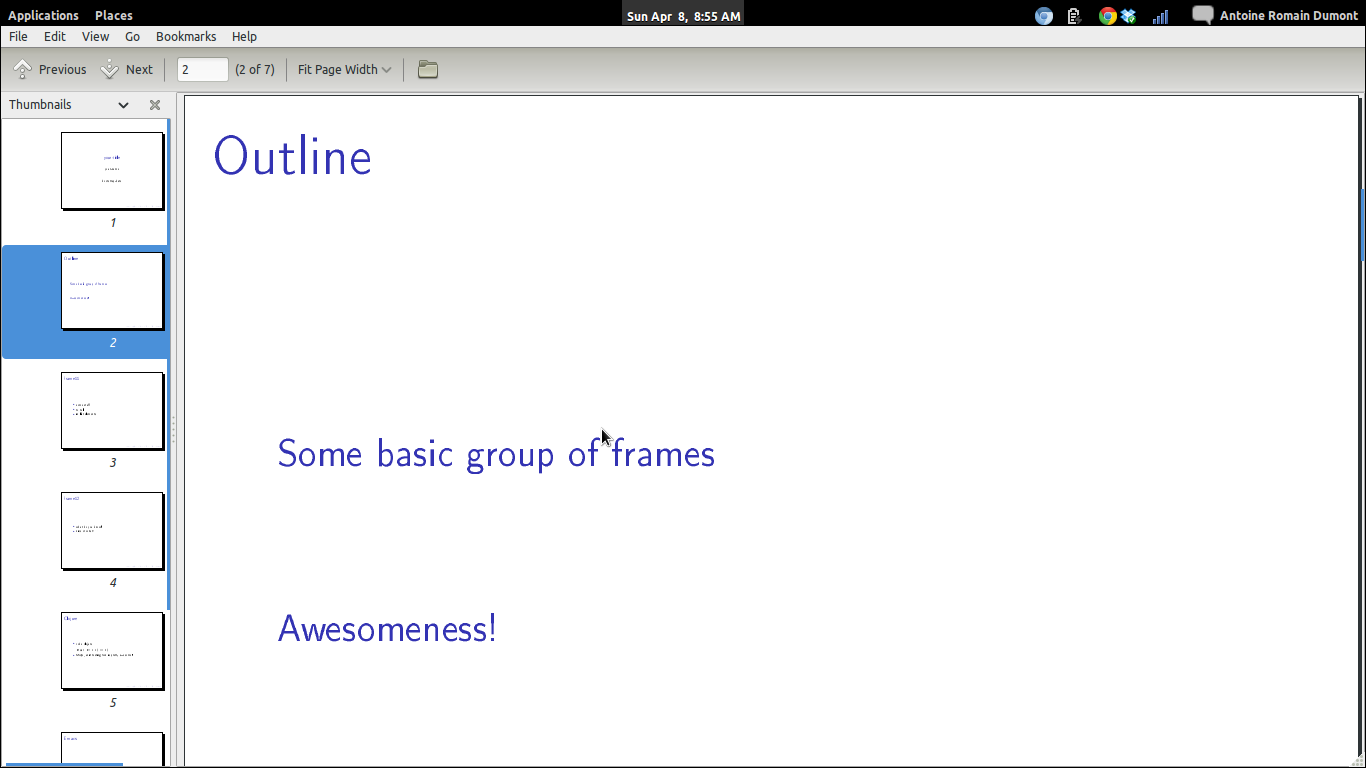
\includegraphics[width=.9\linewidth]{./org-beamer-examples/outline.png}
\subsection{Frame 1}
\label{sec-3-5}


\begin{verbatim}
* Some group of frames
** frame11
*** some stuff
*** to tell
*** in list elements
\end{verbatim}

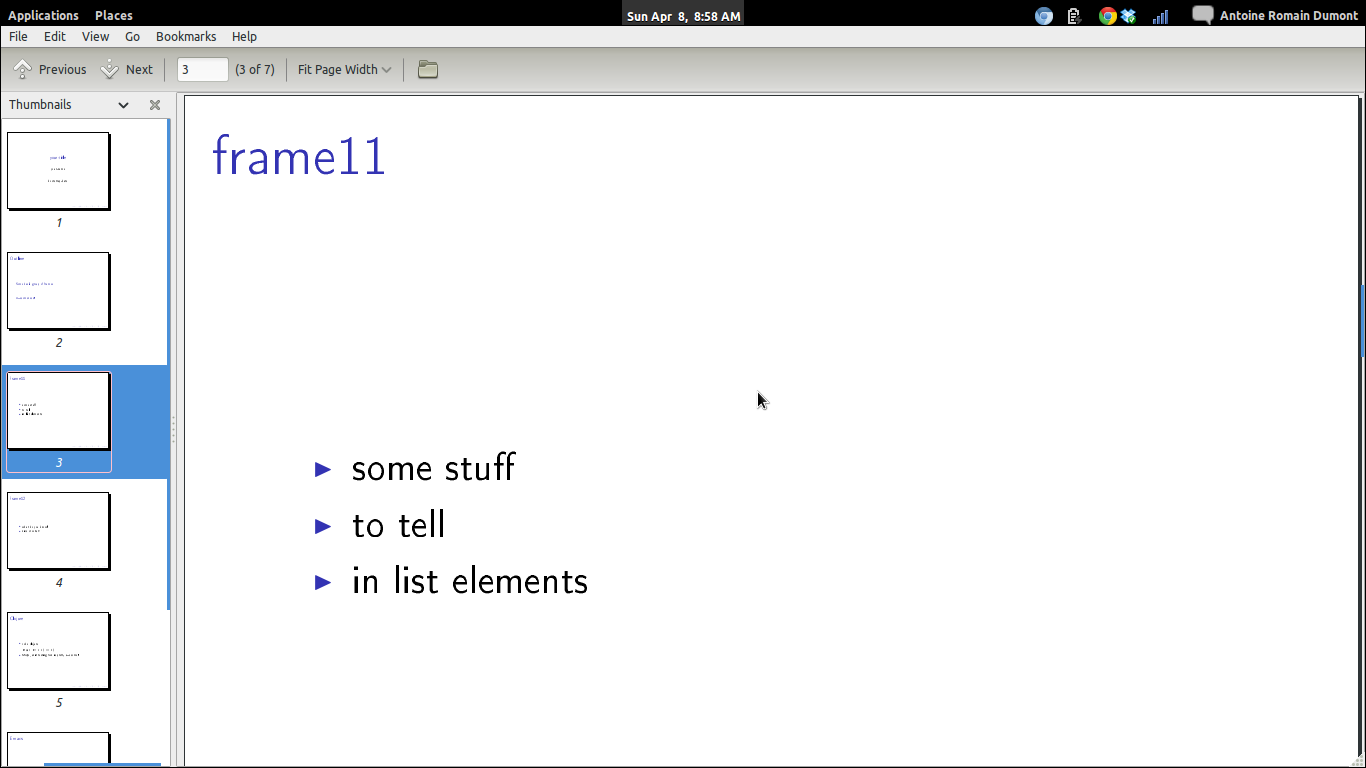
\includegraphics[width=.9\linewidth]{./org-beamer-examples/frame-11.png}
\subsection{Frame 2}
\label{sec-3-6}


\begin{verbatim}
** frame12
*** what do you know!
*** nice or what?
\end{verbatim}

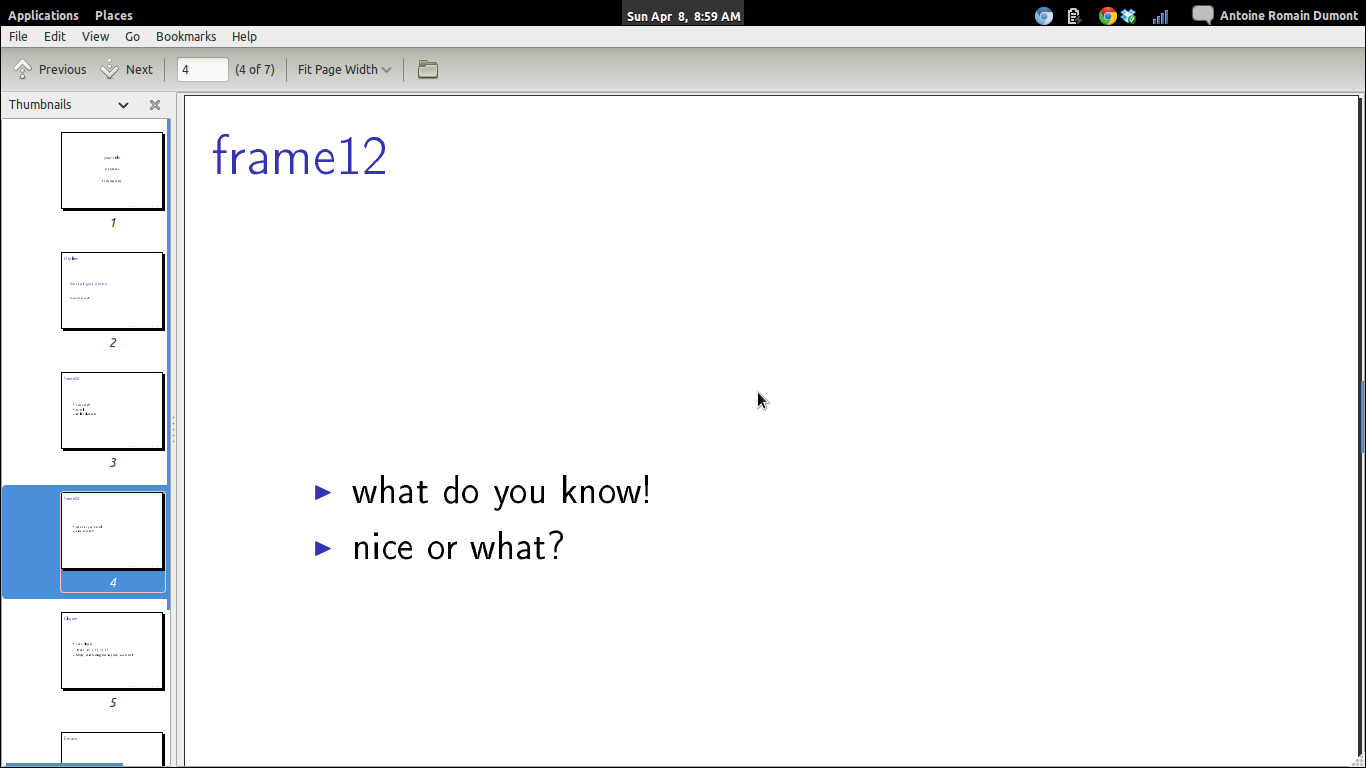
\includegraphics[width=.9\linewidth]{./org-beamer-examples/frame-12.png}
\subsection{A frame about clojure in another group}
\label{sec-3-7}


\begin{verbatim}
* Awsomeness!
** Clojure
*** code clojure
*** /Midje/, unit testing fwk is pretty awesome!
\end{verbatim}

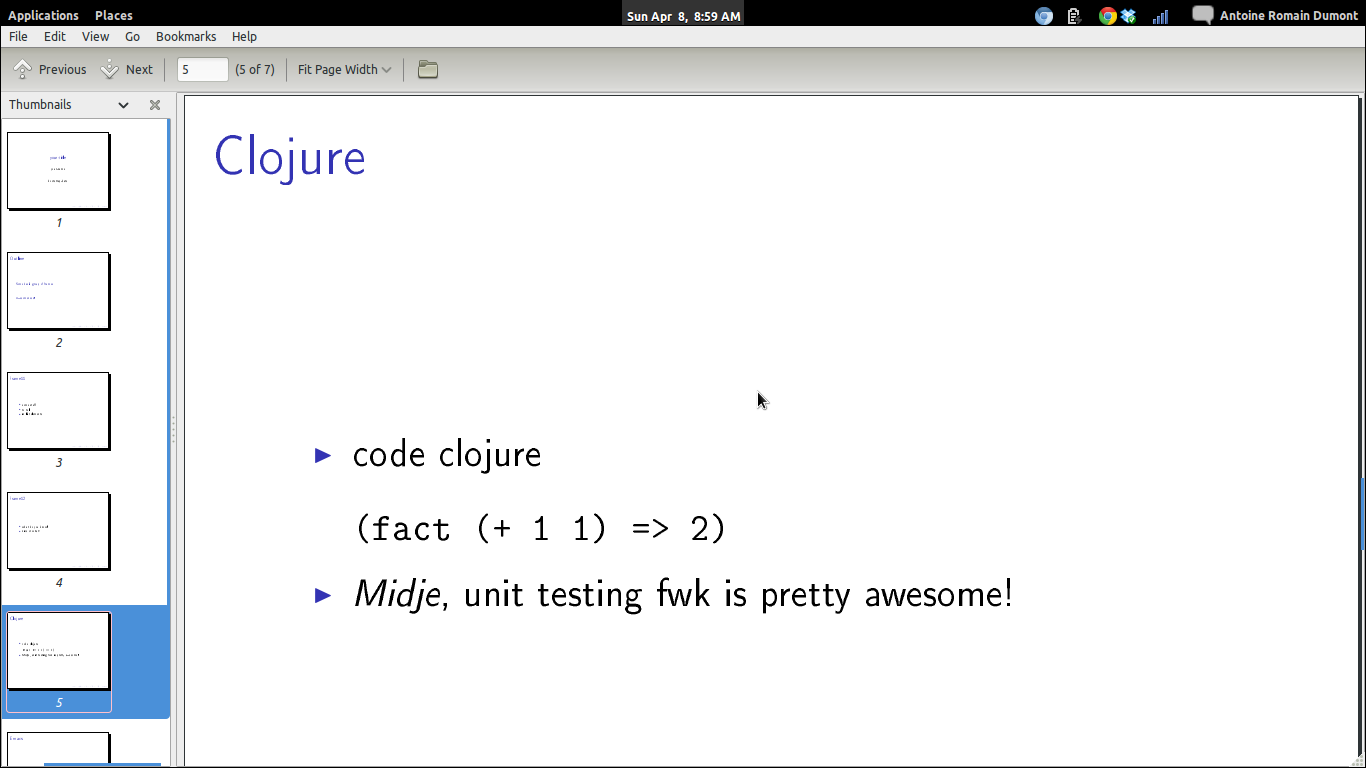
\includegraphics[width=.9\linewidth]{./org-beamer-examples/frame-clojure.png}
\subsection{About emacs}
\label{sec-3-8}


\begin{verbatim}
** Emacs
*** It's pretty cool too!
\end{verbatim}

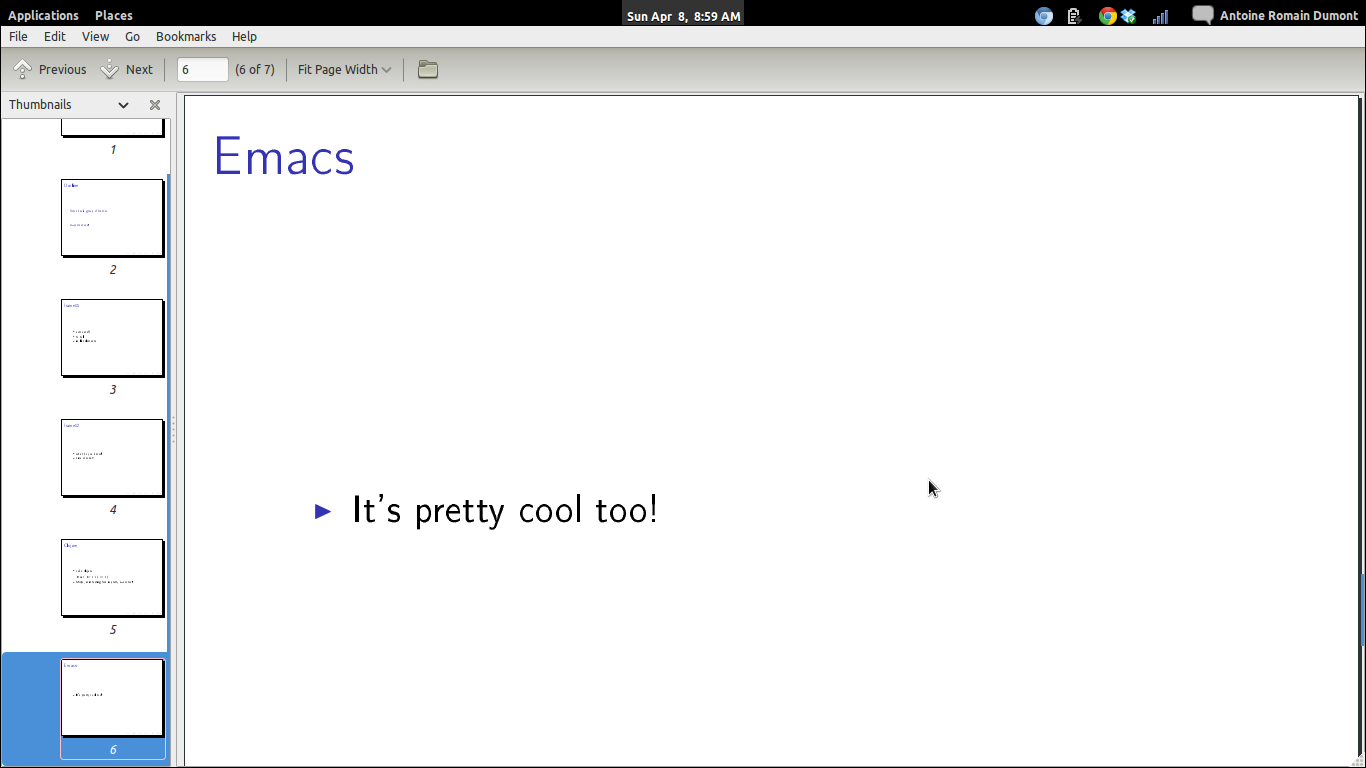
\includegraphics[width=.9\linewidth]{./org-beamer-examples/frame-emacs.png}
\subsection{Org}
\label{sec-3-9}


\begin{verbatim}
** Org-mode with beamer
*** rocks as we can present                                           :BMCOL:
:PROPERTIES:
:BEAMER_col: 0.5
:END:
*** in columns
*** and as always
:PROPERTIES:
:BEAMER_col: 0.5
:END:
[[./clj-pink.png]]
*** include images
\end{verbatim}

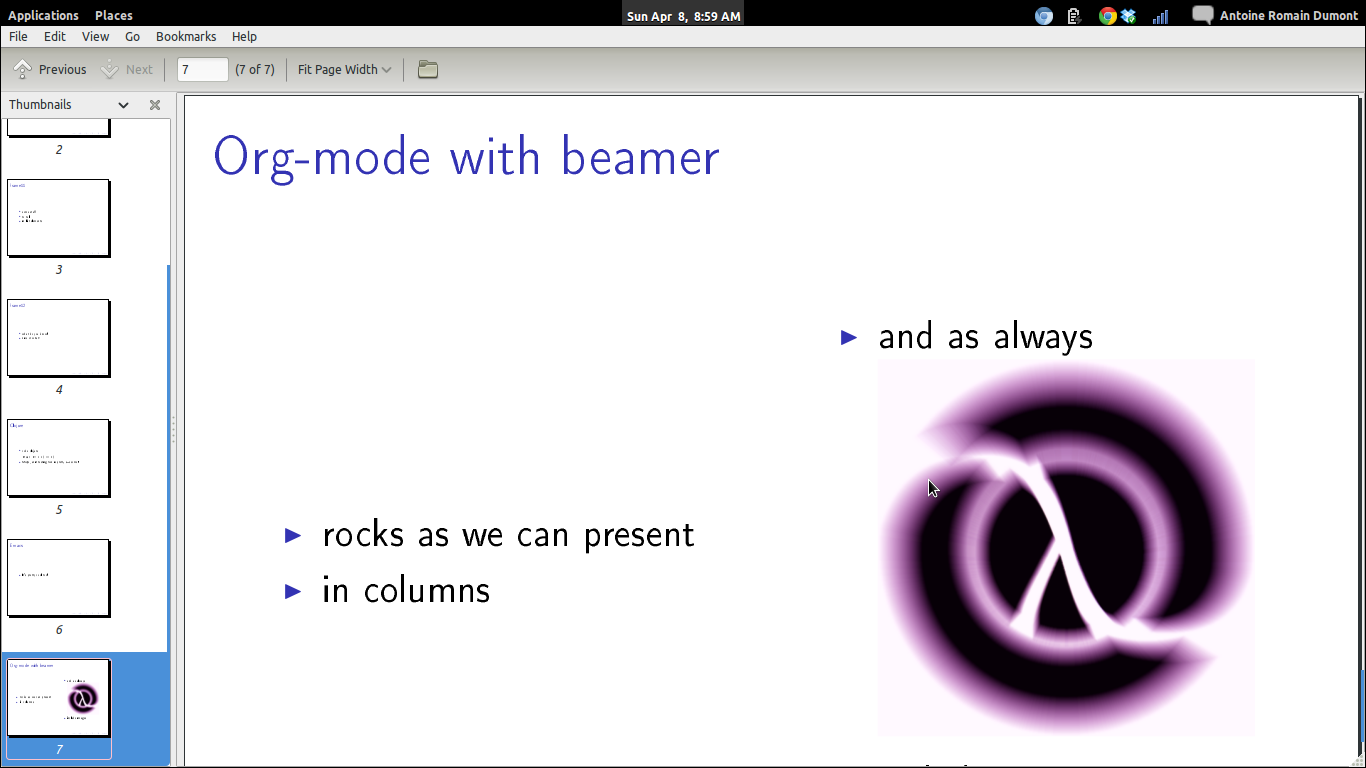
\includegraphics[width=.9\linewidth]{./org-beamer-examples/frame-org.png}
\section{Launch the export}
\label{sec-4}


C-c C-b will launch a buffer with the options for exporting in the format you want!


\begin{center}
\begin{tabular}{ll}
\hline
 C-c C-b d  &  compile in latex, then export to pdf and open it.  \\
\hline
\end{tabular}
\end{center}
\section{And that's it}
\label{sec-5}

\end{document}
